\section{System Architecture}
\label{sec:architecture}

\begin{figure}[t]
    \centering
    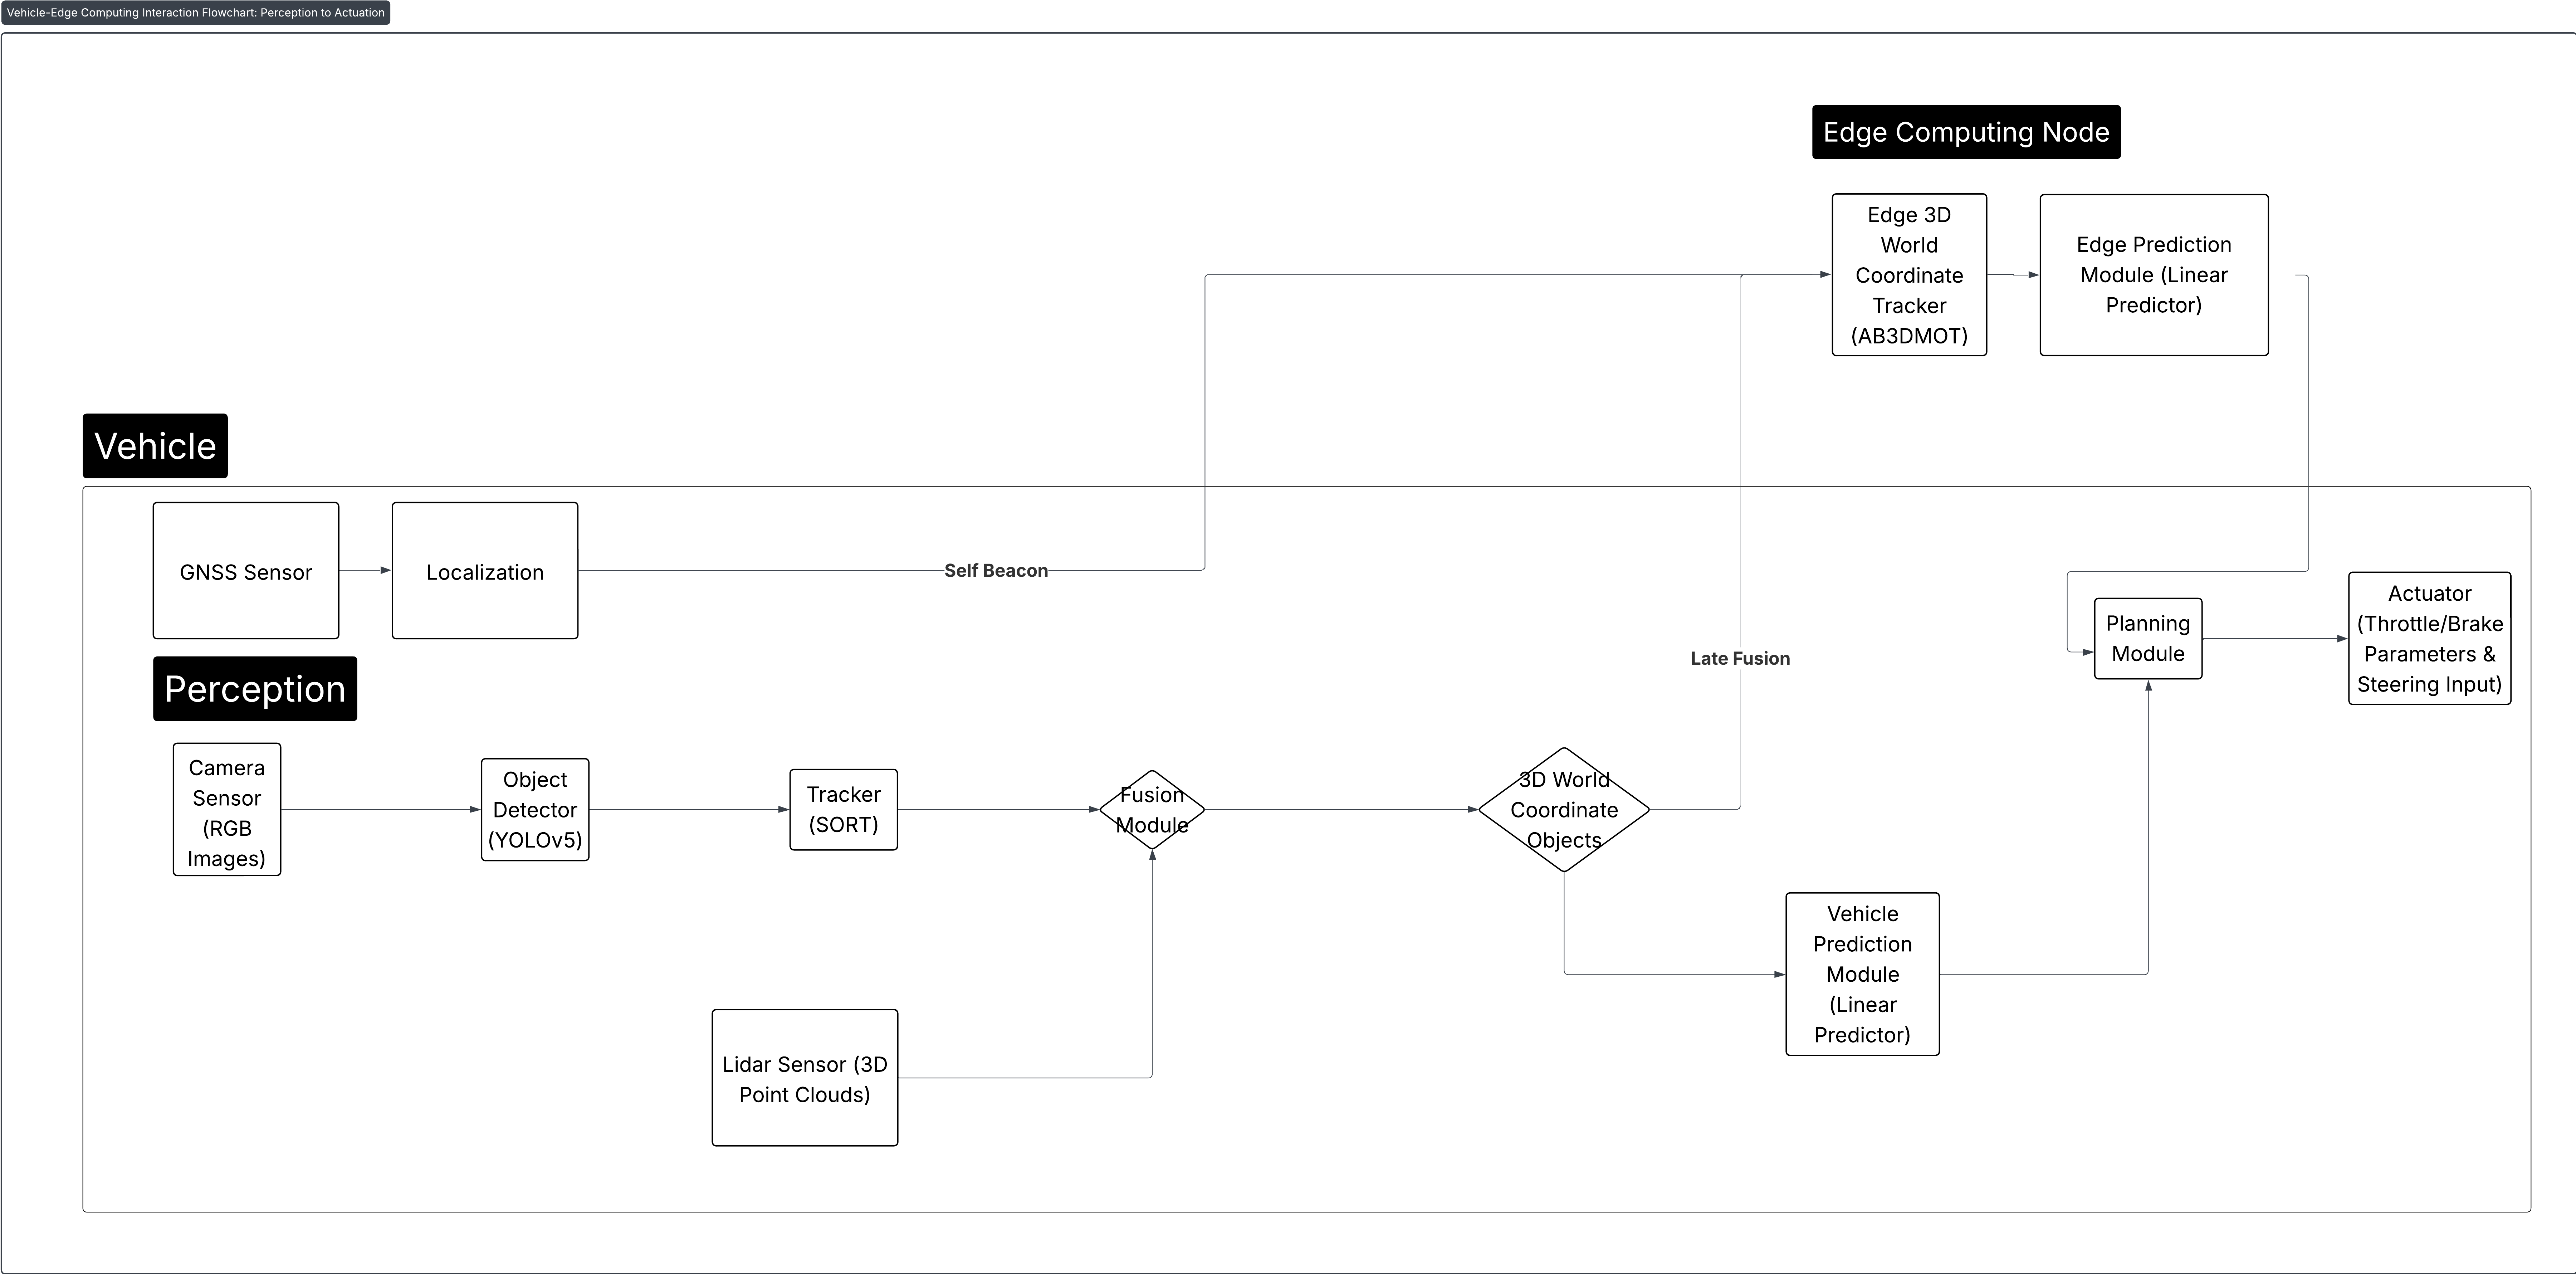
\includegraphics[width=\columnwidth]{../docs/md_files/images/system_architecture.png}
    \caption{Edge cooperative world-model pipeline.  Each CAV encodes
      LiDAR into a compressed post-backbone BEV feature (17\,KB) and
      uploads via 5G Uu.  The edge runs WorldFusion (Where2Comm)
      attention fusion, AB3DMOT tracking, and MTR trajectory prediction.
      The adaptive controller selects which agents and objects to
      process within the 100\,ms planner deadline.}
    \label{fig:system_overview}
\end{figure}


The edge pipeline processes each tick in four sequential stages:
fusion, detection, tracking, and prediction.  We instantiate each
stage with a specific model and measure its per-stage cost scaling
on an NVIDIA RTX~4080~SUPER (16\,GB).

\subsection{Intermediate Fusion: WorldFusion (Where2Comm)}

Each CAV runs a PointPillars~\cite{lang2019pointpillars} encoder
locally, producing a BEV feature tensor.  After post-backbone
compression (NaiveCompressor at 256$\times$, reducing the per-vehicle
payload from $\sim$10\,MB to $\sim$17\,KB), compressed features are
uploaded to the edge via 5G Uu.  The edge decompresses and fuses using
Where2Comm~\cite{hu2022where2comm} spatial attention, which computes
pairwise confidence-weighted attention maps over BEV cells.

Fusion cost scales linearly in $K$ (the number of agents after input
filtering): from 3.5\,ms at $K=4$ to 29.5\,ms at $K=32$ for
Where2Comm attention.  Simple maxout pooling is 20--40$\times$ faster
but sacrifices detection quality.

\subsection{Detection}

The fused BEV feature is passed through classification and regression
heads (shared with the per-agent encoder) to produce 3D bounding
boxes via anchor-based decoding and NMS.  Detection cost is near-constant
in $N$ ($\sim$1\,ms) because it operates on the single fused feature
map.

\subsection{Tracking: AB3DMOT}

We use AB3DMOT~\cite{ab3dmotTracker2020} with vectorized Kalman
predict/update (replacing the original serialized per-track loop with
batched \texttt{einsum} operations), yielding a 1.8--1.9$\times$
speedup.  Additional modifications include tightened confirmation
gates, duplicate filtering, and kinematic gating.

Tracking cost scales linearly in the number of detected objects $M$:
$c_{\mathrm{track}} \approx 0.7\,\text{ms} \times M$.  Through
$N=32$ agents, tracking remains the cheapest stage.

\subsection{Prediction: MTR}

We selected Motion Transformer (MTR)~\cite{shi2022mtr} over
SMART~\cite{wu2024smart} after benchmarking both on OPV2V data.
SMART's 143\,ms constant-time inference alone exceeds the 100\,ms
deadline.  MTR achieves 4.5\,m ADE and 9.4\,m FDE at 57\,ms.
SMART yields 42.7\,m ADE and 50.3\,m FDE at 137\,ms on the same
data, reflecting a domain gap (SMART was trained on Waymo, not
CARLA-based data).

MTR runs in single-call mode at the edge: one forward pass per tick
over all tracked objects, producing 25-step multi-modal trajectories.
Compared to the per-CAV invocation used in CMP~\cite{cmp2024},
single-call inference is 1.3$\times$ faster with statistically
indistinguishable ADE (4.13\,m vs.\ 4.10\,m).

Prediction cost decomposes as $c_{\mathrm{base}} + c_{\mathrm{marginal}}
\times |\{i : x_i = 1\}|$, where $c_{\mathrm{base}} \approx 25\,$ms
(model load, map encoding) and $c_{\mathrm{marginal}} \approx 1.5\,$ms
per additional object.

\subsection{Cost Model}

The total per-tick pipeline cost is:
\begin{equation}
  C(K, \mathbf{x}) = c_{\mathrm{filt}}(N) + c_{\mathrm{fuse}}(K)
    + c_{\mathrm{det}} + c_{\mathrm{track}}(M)
    + c_{\mathrm{pred}}(\mathbf{x}) + c_{\mathrm{oh}}
  \label{eq:cost}
\end{equation}
where $c_{\mathrm{filt}}(N)$ is the input filter cost ($\sim$0.05\,ms
per agent), $c_{\mathrm{fuse}}(K) \approx 1.0\,\text{ms} \times K$,
$c_{\mathrm{det}} \approx 1.0\,$ms, $c_{\mathrm{track}}(M)
\approx 0.7\,\text{ms} \times M$, $c_{\mathrm{pred}}(\mathbf{x})$
per above, and $c_{\mathrm{oh}} \approx 2\,$ms is scheduling overhead.
Coefficients are calibrated from per-stage profiling
(\cref{sec:eval}).

\subsection{Static Pipeline Scaling}

\Cref{tab:stage_latency} shows measured per-stage latency vs.\ $N$
for the static (no adaptation) configuration.  The pipeline first
exceeds 100\,ms at $N=16$, reaching 184\,ms at $N=64$.  Fusion and
prediction dominate; tracking remains sub-linear through $N=64$.
